\documentclass[twocolumn]{article}

\usepackage{graphicx}

\usepackage{color}
\usepackage{listings}
\usepackage{caption}
\usepackage[affil-it]{authblk} % Affilation


%%%%%%%%%%-----TODOS
\setlength{\marginparwidth}{2cm}
\usepackage[obeyFinal]{todonotes}

%%%%%% OWN Pseudocode style
\newcounter{nalg}[section]
\renewcommand{\thenalg}{\thesection .\arabic{nalg}}
\DeclareCaptionLabelFormat{algocaption}{Algorithm \thenalg}
\lstnewenvironment{algorithm}[1][]
{   
    \refstepcounter{nalg}
    \captionsetup{labelformat=algocaption,labelsep=colon}
    \lstset{
        mathescape=true,
        frame=tB,
        numbers=left, 
        numberstyle=\tiny,
        basicstyle=\scriptsize, 
        keywordstyle=\color{black}\bfseries\em,
        keywords={,input, output, return, datatype, function, if, else, foreach, while, begin, end, or, }
        numbers=left,
        xleftmargin=.04\textwidth,
        #1
    }
}
{}

\usepackage{amsmath}
%%%%%%% Make it possible to write over a leftrightarrow

\makeatletter
\newcommand{\xleftrightarrow}[2][]{\ext@arrow 0099\Leftrightarrowfill@{#1}{#2}}
\makeatother

%%%%%% SPECIFY own MOD
\newcommand{\Mod}[1]{\ (\mathrm{mod}\ #1)}

%%%%%%%%%%-----REFERENCES
\usepackage[hidelinks]{hyperref}	% Makes references clickable

\graphicspath{{images/}}



\title{Concolic testing: An overview of the used techniques and its limits}
\author{Matthias Gabriel}
\affil{University of Applied Sciences Rapperswil\\Supervisor Prof. Peter Sommerlad\\Seminar HS2019}
\date{\today}


\begin{document}
\maketitle

\begin{abstract}
There exist certain classes of errors, which are hard to reason about in static code analysis and it's difficult and time consuming to manually write tests that cover every possibility.
In recent years different approaches that require the program to execute, such as fuzzing or symbolic execution, have arisen.
In symbolic execution instead of using concrete values, the program will be executed on so-called symbolic values.
This article summarizes the basic knowledge that is required to understand how concolic testing works and presents deeper explanations about KLEE, which just is one of many solutions.
Because an execution purely based on symbolic values is sometimes not possible, concolic execution, a mixture of concrete and symbolic execution can be performed and will often be referred to as concolic testing.
Based on concrete examples it's shown which errors can be detected and where manually written tests are still required.
\todo{write abstract}
\end{abstract}
\section{Introduction}
In recent years many different publications were published in the field of symbolic and concolic execution. 

The primary purpose of this article is to give an overview of the techniques which are used in symbolic and concolic execution engines.
It mainly focuses on the specific engine KLEE \cite{Cadar:2008:KUA:1855741.1855756}, but many of the presented concepts are found in numerous other applications.
The understanding of these techniques is very important to understand the advantages and disadvantages that arise from using automated testing engines.

The second purpose is to analyse how KLEE behaves in relation to other testing approaches.

Section \ref{section:contraint_solvers} contains some insights about constraints solvers, which are used heavily in symbolic and concolic execution.
Section \ref{section:symbolic_execution} section presents the basics of symbolic execution.
Section \ref{section:concolic_testing} finally focuses on concolic testing based on the example of KLEE \cite{Cadar:2008:KUA:1855741.1855756}. 
Section \ref{section:handwritten_vs_generated_tests} contains a short breakdown of my opinion where concolic testing is helpful and where it's limits are.
\section{Constraint Solvers}\label{section:contraint_solvers}
A constraint solver is a program that tries to find a valid solution to a formulated logical problem. 
There are many different types of constraint solvers, that are sometimes generic and sometimes very specific to a problem domain.
In this section you will find an overview over the two types of constraint solvers that are used in KLEE to solve the logical problems, that arrise during concolic execution.
\subsection{Satisfiability Solvers}
A SAT solver basically tries to find a solution, an assignment of all variables so that the formula is true, to a specified boolean formula. All modern SAT Solvers additionally return a specific assignment if possible or otherwise specify that the formula is not satisfiable.

As an example take the following formula as an input $A \land \lnot B$ there's only one variable assignment where the formula evaluates to true, namely A = true and B = false.

An unsatisfiable example would be the following formula: $A \land \lnot B \land (\lnot A \lor B)$.  There's no possibility how to assign boolean values to A and B so that the formula evaluates to true as shown by table \ref{table:unsat_truth_table}, therefore its unsatifable.
\begin{table}[!htbp]
\begin{adjustbox}{width=\columnwidth}
\begin{tabular}{ |c|c|c|c|c| } 
 \hline
 $A$ & $B$ & $\lnot B$ & $\lnot A \lor B$ & $A \land \lnot B \land (\lnot A \lor B)$ \\ 
 \hline
 True & True & \highlight{False} & True & False \\ 
 True & False & True & \highlight{False} & False\\ 
 \highlight{False} & True & \highlight{False} & True & False\\ 
 \highlight{False} & False & True & True & False\\ 

 \hline
\end{tabular}
\end{adjustbox}
\caption{Truth table for the unsatisfiable example. The partial expressions that lead to the expression evaluating to false are highlighted.}
\label{table:unsat_truth_table}
\end{table}

To simplify the task, the formula has to meet certain criteria to be allowed as an input to a SAT solver. The most important criteria is that the formula has to be in the conjunctive normal form, hereinafter referred to as CNF. 

In the following paragraph, the rules of CNF will be explained followed by some examples. The next paragraph shows that this restriction to CNF is not a big problem, because it's possible to transform any boolean formula into CNF\cite{Jackson:2004:CFC:2103144.2103160}.
\subsubsection{CNF}
CNF uses variables like $A$ or $B$ which can either be true or false.
These variables are used in literals. Each literal consists of exactly one variable or its negation. It's allowed to use a variable in multiple literals, but only one of the values \{true, false\} can be assigned to a variable, which will be used in the whole formula.

Consider the two example literals: $A$ and $\lnot B$

These literals can be combined to form a clause. Each of the clauses consists of any number of literals that are in a disjunctive relation. 

Let's suppose the following three clauses: 
$$A \lor B$$
$$B \lor \lnot C$$ 
$$C$$
Each formula in CNF consists of any number of clauses which are in an conjuctive relation. For example: $$clauseOne \land clauseTwo \land clauseThree$$\\
The whole boolean formula would therefore be: $$\underbrace{(A \lor B)}_{clauseOne} \land \underbrace{(B \lor \lnot C)}_{clauseTwo} \land \underbrace{(C)}_{clauseThree}$$\\

If a boolean formula is not in the CNF it's necessary to convert it before entering into the SAT solver. For example the boolean formula $\lnot(A \lor B) \lor C$ can be converted into ($\lnot A \lor C) \land (\lnot B \lor C)$

There are different kinds of special clauses:
\begin{itemize}
\item empty clause
\item unit clause
\item binary clause
\end{itemize}
The empty clause contains no literal and is in literature denoted with different symbols. In this publication, an uppercase lambda $\Lambda$ will be used as suggested by Gomes et al \cite{Gomes2008SatisfiabilityS}.
The empty clause always evaluates to false, because there is no possibility to assign a variable which lets the clause evaluate to true.

The unit clause contains exactly one literal. This literal either contains a variable or its negation as described before. 
The clauses $A$ and $\lnot A$ are both unit clauses. 
The unit clause is a special case because its possible to deduce the value of the variable used in the unit clause.
If a CNF formula should evaluate to true and contains a unit clause the unit clause must also evaluate to true. 
This property will be heavily used by the SAT solver.

Consider the example clauses used above. In clause $A$ the variable $A$ has to be true and in the other example, $\lnot A$ the variable $A$ has to be false.

The binary clause contains exactly two literals. At a first glance, this does not look very special at all, but binary clauses allow powerful optimizations. As soon as one of the two variables gets assigned it's possible to deduct the value of the other variable. This, for example, allows it to efficiently track the event when a variable can be deducted.
\subsubsection{DPLL}

There are many different methods how a SAT Formula can be solved. The most simplistic approach would be to just brute-force the formula and try to evaluate the formula for every possible combination of variables. This works well for a small number of variables but does not scale, because the computation time increases exponentially. In this chapter, the method of the DPLL procedure will be presented. It is the basis for many of the currently used algorithms and fortunately not too hard to understand.

The predecessor of this method was first presented in 1960 by Davis and Putnam \cite{Davis:1960:CPQ:321033.321034} and improved in 1962 by Davis, Logemann and Loveland \cite{Davis:1962:MPT:368273.368557}, hence the name DPLL which consists of the initials of the inventors.

Even though the worst case still requires exponential time, normally these algorithms provide massive computational benefits. In this publication, the recursive version of the algorithm will be used because it's much easier to understand some of the key ideas. Note that the algorithm also exists in iterative versions, which are able to reduce the memory usage \cite{Gomes2008SatisfiabilityS}.

The algorithm will be represented by two parts of pseudo-code algorithms \ref{algDPLLRecursive}, \ref{algUnitProgagate}.

The algorithm DPLLRecursive shows the general structure of the approach, but the algorithm UnitPropagate actually is similarly important.

\begin{algorithm}[caption={DPLLRecursive}, label={algDPLLRecursive}]
 input: $F$: boolean formula in CNF-Form
	$\rho$: assignment of variables
 output: assignment that satisfies F or 
	UNSAT if no assignment is possible
 begin
   $(F, \rho)$  $\gets$ UnitPropagate
   if $\Lambda \in F$
       return UNSAT
   if $F = \emptyset$
       return $\rho$
   $l \gets$ a literal not assigned by $\rho$
   $result \gets$ DPLLRecursive($F \cup \{l\}, \rho$)
   if $result \neq UNSAT$
       return result
   return DPLLRecursive($F \cup \{\lnot l\}, \rho$)
\end{algorithm}


\begin{algorithm}[caption={UnitPropagate}, label={algUnitProgagate}]
 input: $F$: boolean formula in CNF-Form
	$\rho$: assignment of variables
 output: $F$: updated boolean formula
	$\rho$:updated assignment of variables
 begin
   while $F$ contains no empty Clause
   and there exists a UnitClause $xClause$
       $xLiteral \gets$ the only literal of $xClause$
       while there exists an $yClause$ in $F$
       which contains an $xLiteral$
           $F \gets F \setminus \{yClause\}$     
       while there exists an $zClause$ in $F$
       which contains an $\lnot xLiteral$
           $newZClause \gets zClause \setminus \{\lnot xLiteral\}$
           $F \gets (F \setminus \{zClause\}) \cup \{newZClause\}$
       $\rho \gets \rho \cup \{xLiteral\}$
   return $(F, \rho)$
 end
\end{algorithm}


First, the unit propagation is executed, after that it's checked if either of the base cases is reached. 
There are only two base cases. Either the formula contains no more clauses that result in a satisfying formula (as shown in lines 9-10) or the formula contains an empty clause that results in UNSAT (as shown in lines 7-8).

The next step (line 11), also called branching step, selects the literal $l$, which should be eliminated in the next recursion.

The last step of the DPLLRecursive is to call itself twice with new input. In one case a new unit clause with the selected literal $l$ is added to the formula (line 12), in the other case the unit clause with the negation of the literal, $\lnot l$, is added (line 15).

The step where the first recursion ends in UNSAT and returns to the base is called backtracking. In the recursive version, this is very simple because there's literally nothing to be done. However in the iterative version, that is used in practice, backtracking can be very sophisticated.

The second part of the algorithm, called UnitPropagate, which is the first step of the DPLL algorithm, will try to assign values to all variables, which can be deducted.

The easiest way to determine the value of a variable is if there is any unit clause in the formula. Because CNF defines that every clause has to be true by itself, the clause and the literal have to be true as well.

Consider the following example: Suppose the unit clause $A$ which is part of the formula, the value true can be assigned to the variable A. On the other hand, suppose the unit clause $(\lnot A)$, the value false can be assigned to the variable A.

After a specific value was assigned to the variable the formula can be updated to reflect the changes. 

As a first step, all clauses that contain the same literal (lines 8-9) have to be removed, as these clauses automatically evaluate to true. 

The second step is to remove all occurrences of the negated literal from all clauses (lines 10-11). This step is possible because the negated literal will always evaluate to false and an $\lor false$ combination is redundant.

This reduction can result in new unit clauses, which then will be propagated until no more feasible clauses can be found or an empty clause $\Lambda$, which leads to an unfeasible formula, is constructed.

\begin{figure}[H]
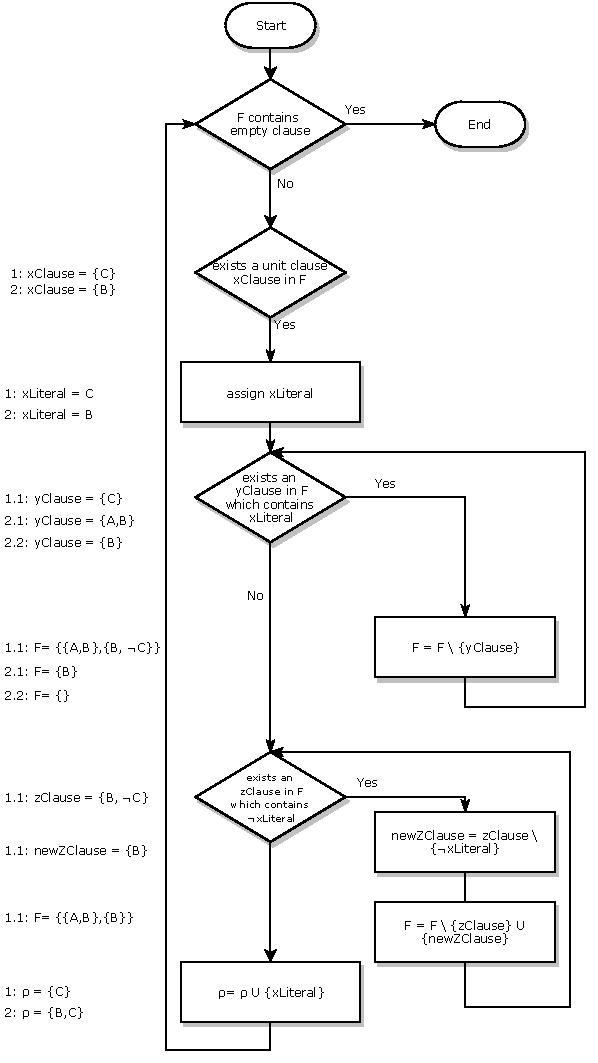
\includegraphics[width=\columnwidth]{unitpropagate}
\centering
\caption{Flowchart of the unit propagate algorithm as desribed in algorithm \ref{algUnitProgagate}.\\ Annotated with the actual values that are assigned for the input $F=(A \lor B ) \land (B \lor \lnot C) \land (C)$ and $\rho = \{\}$. The number on the left side is representing the current iteration.}
\label{fig:unitpropagate}
\end{figure}


\subsubsection{Improvements of today's SAT solvers}
The key differences between the original DPLL Algorithm and currently developed SAT solvers lie in the improvement of either the branching selection of the literal, the backtracking after a branch ends in an UNSAT state and some improvements to the unit propagation.
\todo{Some more details}
\subsection{Satisfiability Modulo Theories Solvers}
In relation to the Satisfiability Solvers, the Satisfiablity Modulo Theories solvers, short SMT solvers, operate on a higher logical level. Because it is often time consuming to formulate your domain specific problem as a boolean formula and transform it into CNF a new class of solvers was defined which tries to overcome this restriction. In this section an overview over how STP \cite{Ganesh:2007:DPB:1770351.1770421}, which is used in KLEE and other tools, works is given.
\todo{maybe add/research something more about first order theories}
In contrast to SAT solvers, STP is able to solve decision problems that contain bit-vectors and arrays. Which in practise allows us to reason about various data types such as integers, integers are principally bit vectors and also some datastructures like lists and arrays.

As an input STP allows the following operations, which can be grouped in the following way:
\begin{itemize}
\item \textbf{logical and boolean} Constant Values TRUE and FALSE, variables with a boolean value, any boolean operator\footnote{such as $\lor$,$\land$, $\Rightarrow$, etc}, bitwise boolean operators
\item \textbf{mathematic operations} Left and right shifts, addition, multiplication, unary minus, division, modulo, relational operators
\item \textbf{others} Array read, array write,  extraction of bit-vectors\footnote{$x[i:j]$ is the extraction of the bytes between $i$ and $j$ of $x$ as described in\cite{Ganesh:2007:DPB:1770351.1770421}}, concatenation of bit-vectors\footnote{The concatenation of two bit-vectors $x_{[n]}$ and $y_{[m]}$ is expressed as $x \circ y$ and returns a new vector $z_{[m+n]}$ of length $m+n$ as described in \cite{Ganesh:2007:DPB:1770351.1770421}}
\end{itemize}
STP was specifically developed with focus on software analysis projects, because there are often extremely large constraint problems involved. In relation to other SMT solvers STP focuses on reducing the size of a quantifier-free first order logic problem, before it will be converted into conjunctive normal form and solved by a SAT solver. This procedure allows it to benefit from the heavely engineered and therefore very fast SAT solvers. Other SMT solvers apply the theory specific decision procedures not until in the included SAT solver, which often leads to problems with the SAT specific optimizations. The architecture of STP is visualized in the figure \ref{fig:spt_architecture}.

\todo{add some more content about the "architecture" / flow of STP}
\todo{add more content about the general working of STP, especially the array refinement}

To reduce the size of a problem it applies optimations specific to bit-vector and array theory.
\begin{figure}
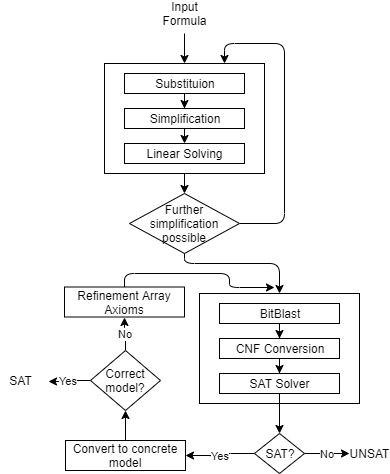
\includegraphics[width=\linewidth]{SPT_architecture}
\centering
\caption{SPT Architecture}
\label{fig:spt_architecture}
\end{figure}
In the original paper\cite{Ganesh:2007:DPB:1770351.1770421} there are two of these optimizations discussed. The first optimization is an "on-the-fly solver for mod-$2^n$ linear arithmetic" which is embedded in STP. 

When reasoning about fixed length bit-vector arithmetic this part of the program tries to reason about parts of the bit-vector equality system.
The idea is to use the property of a such a vector that you can always calculate in $\mod{2^b}$ where is b is the length of the bit-vector.

There exists a mathematical theorem in basic number theory which can be used to determine if a solution to an equation exists if it is$\mod{2^b}$:
$$\sum_{i=1}^{n} a_ix_i = c_i  \Mod{2^b}$$
$$gcd(a_1,...,a_n,2^b) | c_i$$
The equation is only solvable if the greatest common divisor, also known as gcd, is a divisor of every $c_i$.\
Lets assume the following equality system where all variables are bit-vectors with length 3, $b$ is therefore 3:
TODO replace system with own example
$$3x+4y+2z=0 \Mod{2^3}$$
$$2x+2y+2=0  \Mod{2^3}$$
$$2x+4y+2z=0 \Mod{2^3}$$
If the $gcd$ of two numbers is $a$ and $m$ is 1, $a$ has per definition a multiplicative inverse in mod $m$. In this particular case $m=2^b$. This property is necessary, because one of the variables needs to be isolated and therefore multiply with the inverse\footnote{This is neccessary because division in modular arithmetic is defined as the multiplication of the inverse and therefore only works for numbers that have an inverse}.
The algorithm chooses the first equation and tries to find an $a_i$ where $gcd(a_i,2^3) = 1$ is true.

In the example the the algorithm selects $a_1$ which has the value $3$, therefore $x$ can be isolated in the first equation.
The first step is to multiple with the multiplicative inverse of 3 in$\mod{2^3}$ which is also 3.
$$3x+4y+2z = 0 \Mod{2^3} \mid \text{isolate 3x}$$
$$\Leftrightarrow 3x=-4y-2z  \Mod{2^3}  \mid \text{normalize to mod8}$$
$$\Leftrightarrow 3x=4y+6z  \Mod{2^3}  \mid \text{multiple with 3}$$
$$\Leftrightarrow x=12y+18z \Mod{2^3}  \mid \text{normalize to mod8}$$
$$\Leftrightarrow x=4y+2z \Mod{2^3}$$
After $x$ is isolated, it's possible to substitute each $x$ in the original equality system with $4y+2z$ and normalize to$\Mod{2^3}$
$$2(\underbrace{4y+2z}_{x})+2y+2=0 \Mod{2^3} \Leftrightarrow 2y + 4z + 2 = 0\Mod{2^3} $$
$$2(\underbrace{4y+2z}_{x})+ 4y + 2z = 0 \Mod{2^3} \Leftrightarrow 4y + 6z = 0\Mod{2^3} $$
There are no longer any ${a_i}$ in these equalities, that have an $gcd(a_i,2^3) = 1$ and therefore no further variable can be isolated.

The algorithm then searches the coefficent $a_i$ which is the smallest over the whole system and chooses the belonging equality.
After the smallest $a_i$ is choosen the whole system is devided by it and the bit with the highest order is dropped.

A whole new equality system is formed with linear vectors length $b-1$, in the example two.
The new variables are named $y[1:0]$ and $z[1:0]$ to signal that they represent the bits 1 to 0 of the regarding variable.
$$y[1 : 0] + 2z[1 : 0] + 1 = 0 \Mod{2^2}$$
$$2y[1 : 0] + 3z[1 : 0] = 0\Mod{2^2}$$
Now the first step of isolation a variable $x_i$ with a coefficient $gcd(a_i, 2^b)=1$ is repeated.
$$y[1 : 0] + 2z[1 : 0] + 1 = 0 \Mod{2^2}\mid \text{isolate y[1:0]}$$
$$\Leftrightarrow y[1 : 0] = -2z[1 : 0] -1 \Mod{2^2} \mid \text{normalize to mod4}$$
$$\Leftrightarrow y[1 : 0] = 2z[1 : 0] +3 \Mod{2^2}$$
After isolating $y[1 : 0] $ it's allowed to substitute each $y[1 : 0] $ in the original equality system with $2z[1:0]+3$
$$2(\underbrace{2z[1:0]+3}_{y[1:0]}) + 3z[1 : 0] = 0\Mod{2^2} \mid \text{normalize to mod4}$$
$$\Leftrightarrow 3z[1:0] + 2 = 0 \Mod{2^2}$$
In the last iteration $z[1:0]$ will be isolated because the $gcd(3,2^2) = 1$. The inverse of 3 in$\mod{2^2}$ is 3.
$$3z[1:0] + 2 = 0 \Mod{2^2} \mid \text{isolate 3z[1:0]}$$
$$\Leftrightarrow 3z[1:0]=-2  \Mod{2^2}   \mid \text{normalize to mod4}$$
$$\Leftrightarrow 3z[1:0]=2  \Mod{2^2}   \mid \text{multiple with 3}$$
$$\Leftrightarrow z[1:0]=6  \Mod{4}  \mid \text{normalize to mod4}$$
$$\Leftrightarrow z[1:0]=2  \Mod{4}$$
Because a solution was found it can concluded that the original equation system is satisfiable.
The original system can be transformed into $$(x = 4y + 6z) \land (y[1 : 0] = 2z[1 : 0] + 3) \land (z[1 : 0] = 2)$$ and forwarded to the SAT solver.

How SMT solvers work in comparison to SAT solvers.\todo{cleanup}
Especially how the STP \cite{Ganesh:2007:DPB:1770351.1770421} (used in KLEE and other tools) works.
Basically by transforming the input and solve the result of the transformation, if neccessary, with a SAT solver.
Description of Bit-Vector Arithmentic used in the on-the-fly solver\cite{10.1007/978-3-540-71209-1_28}
STP uses many different algorithms to optimize the formula. In the next section two of these optimizations are described, as an example.
on-the-fly solver for mod-2n linear arithmetic
abstraction refinement heuristics for array expressions 
\section{Symbolic Execution}
Introduction to the topic of symbolic execution and its limits \cite{SurveySymExec-CSUR18} . Information about symbolic execution is also included in nearly all sources listed in the section concolic testing
\section{Concolic Testing} \label{section:concolic_testing}
Concolic execution tries to overcome the restrictions of symbolic execution, that were discussed in \ref{section:symbolic_restrictions}. There are many different approaches to do this, but all trade in some of the completeness to be able to fulfil at least a partial analysis of the program.
Based on KLEE \cite{Cadar:2008:KUA:1855741.1855756} one possible approach to these two problems will be presented in this section.

\subsection{Main approaches of KLEE}
KLEE only works on programs that are first compiled into the LLVM, an assembly language. This is normally done by using the compiler Clang. Clang is currently able to compile C, C++  and Objective-C programs into LLVM.
Each of the states that we saw in the previous examples \ref{fig:sym_example_one} and \ref{fig:sym_tree_loop} has the properties $\sigma$, now called heap, and $\pi$, which is called path condition. Additionally, each state has a register file, a stack, and an instruction pointer. Based on the current instruction that is processed, KLEE either modifies $\sigma$ or $\pi$ as we saw in the previous chapters.

If the statement needs a modification of $\sigma$, the instruction gets mapped into an identitcal symbolic instruction. For most instructions the symbolic execution is trivial. For example the result of an addition of two symbolic values is just the addition of the two values and will not get simplified during the operation. After applying the following instruction the $\%dst$ register contains the expression $Add(\%src0, \%src1)$\footnote{This exact example was originally described in \cite{Cadar:2008:KUA:1855741.1855756}}
$$\%dst = add\text{ }i32\text{ }\%src0,\text{ }\%src1$$
Note however that KLEE executes the operation directly if all input values are concrete and therefore assigns a new concrete value to the variable.\todo{non trivial instructions}
Assume the current variable assignments $a = 5$, $\b = \alpha_b$ and $c=\alpha_c$. If the statement $a = a + 10$ gets executed, the value of $5 + 10$ has to be calculated and leads to $a = 15$, however the statement $b = b + c$ leads to $b = \alpha_b + \alpha_c$

If it is a branching statement, $\pi_{true}$ as well as $\pi_{false}$ are calculated. A duplication of the current state takes place after the two $\pi$ are checked for feasibility in combination with the current path condition.

This process continues until all branches are processed or a defined timer is reached. In smaller applications, it's still possible to reach all possible states and therefore reach completeness. In more complex applications it's required to optimize the scheduling \ref{section:state_scheduling} to reach the best possible coverage of states before the timer hits the defined limit.
\subsubsection{Approach for dangerous operations}\label{section:dangerous_operations}
In addition to branching statements, each potentially dangerous operation, such as pointer dereference, array access, division operations, modulo operations and assert statements, generates a new branch too. With this additional branching step it's possible to automatically check if any input is possible, which results in an invalid operation. This state never has a subtree attached. If the path condition is infeasible the execution stops automatically, before the branching takes place. However, if it's feasible, an error is raised resulting in the cancellation of this subtree. On the other branch, the negative of the condition is added to prevent the error in this state and to be able to continue the analysis of the program.

The only special cases of these dangerous operations are loading and storing operations. KLEE maps every object to a STP specific array. This enables STP to ignore the parts of the state data, which are not directly related to the expression that gets evaluated. Since it could be possible that a "symbolic" pointer refers to different objects, the state will be cloned for each of the objects as soon as the pointer gets dereferenced. With the cloning it can be ensured that in every state the pointer references exactly one specific object. This may seem very pricy, as for each possible object a new state has to be created. However, in reality, semantic pointers to multiple objects rarely happen. 

\subsubsection{State management}
As there are many states created and even hold during the execution, KLEE tries to minimize both the creation time of a new state as well as the memory footprint. It does this by taking advantage of the big redundancy that these states have because they are often related and only differ in some of their properties. To be able to use this redundancy KLEE treats all memory objects as immutable and thus can reuse them as often as required. The consequence of this property is that whenever an object has to be modified it needs to be copied. This process is also called copy-on-write.

\subsubsection{State scheduling}\label{section:state_scheduling}
Even if the states are very slim and efficiently created depending on the order of the computation, the computation engine could be blocked by a single loop, leading to the starvation of other states. Assume a very simplistic depth-first approach that first creates the two related states on every branching condition and after that processes the state that fulfils the branching condition. In the example with a loop \ref{fig:sym_tree_loop} the engine would always process the left child and no output would be generated at all. State C and State G would be constructed but never analyzed and therefore no return statement would be reached.

To prevent this, KLEE implements two different kinds of scheduling algorithms. 

Random Path Selection organises the states in a binary tree, as visualised by the previous examples, but instead of just going depth-first at the current path, the algorithms randomly selects which path to go when traversing the tree. After each execution of a state, the traversing starts at the top again and thus favours unprocessed states that are higher up in the tree as visualized in figure \ref{fig:state_tree_probability}. Because of this, the starvation of states is no longer possible. A nice side effect of this selection is, that the conditions in higher states are smaller and therefore the processing takes less effort.

Coverage-Optimized Search is the second algorithm that is included in KLEE. As its name suggests, it tries to maximize the coverage. It uses different heuristics to determine how probable it is to reach currently uncovered code in the next few steps. After that it randomly selects the branch based on this probability, preferring states with higher probability.
To benefit from the positive features of both algorithms KLEE normally uses them in a round-robin manner. Because the scheduling is very much dependent on the analysed software and another scheduling algorithm may deliver better results, KLEE allows other state scheduling mechanisms to be used.
\begin{figure}
\begin{tikzpicture}[
    grow=down,
  baseline,
  level distance=25mm,
  text depth=.1em,
  text height=.8em,
  scale = 1,
  level 1/.style={sibling distance=11em},
  level 2/.style={sibling distance=10em},
    edge from parent/.style={very thick,draw=blue!40!black!60,
        shorten >=5pt, shorten <=5pt},
    edge from parent path={(\tikzparentnode.south) -- (\tikzchildnode.north)},
    kant/.style={text width=2cm, text centered},
    straight/.style={text width=2cm},
    every node/.style={text ragged, inner sep=2mm},
    pending/.style={rectangle, rounded corners, shade, top color=white,
    bottom color=blue!50!black!20, draw=blue!40!black!60, very
    thick },
    analysed/.style={rectangle, rounded corners, shade, top color=blue!50!black!20,
    bottom color=blue!50!black!40, draw=blue!40!black!60, very
    thick }
    ]

\node[analysed] [rectangle split, rectangle split, rectangle split parts=1, text ragged] {
   	 \textbf{State A}}
child {
	        node[analysed] [rectangle split, rectangle split, rectangle split parts=1, text ragged] {
		\textbf{State B}
	        }
child {
	        node[pending] [rectangle split, rectangle split, rectangle split parts=2, text ragged] {
		\textbf{State F}
		\nodepart{second}
   		0.5
	        }
        edge from parent
            node[straight, right, midway] {1.0}}
        edge from parent
            node[kant, below, pos=.4] {0.5}}
child {
	        node[analysed] [rectangle split, rectangle split, rectangle split parts=1, text ragged] {
		\textbf{State C}
	        }
child {
	        node[pending] [rectangle split, rectangle split, rectangle split parts=2, text ragged] {
		\textbf{State D}		
		\nodepart{second}
   		0.25
	        }
        edge from parent
            node[kant, below, pos=.4] {0.5}}
child {
	        node[pending] [rectangle split, rectangle split, rectangle split parts=2, text ragged] {
		\textbf{State E}
		\nodepart{second}
   		0.25
	        }
        edge from parent
            node[kant, below, pos=.4] {0.5}}
        edge from parent
            node[kant, below, pos=.4] {0.5}};

\end{tikzpicture}
\caption{Binary state tree with the chance to get selected. On the edge the relative chance is given, which is normally either 1 or 0.5 based on the above statement.}
\label{fig:state_tree_probability}
\end{figure}
\subsubsection{Query optimization}
Since KLEE sends many and very complex queries to STP, the computation time of these queries takes the majority of the time when executing an analysis. To reduce the computational time and thus be able to finish the analysis faster or at least cover more states in the same time window, different optimizations are applied before a query gets solved by STP. 
At the start of these optimizations KLEE tries to do arithmetic simplifications($5*\alpha_a + 2*(4-\alpha_a) = 3 * \alpha_a + 8$). These rewritings are always related to exactly one condition of the whole path condition or one variable entry in the memory.

The second and third optimization exploit the additional information that arises from equality constraints. In the so-called Constraint Set Simplification KLEE tries to simplify the whole path condition by replacing symbolic values if such a new equality constraint is added. Previous conditions can often be eliminated or at least simplified. 
Assume the following path condition $\pi = \{\alpha_a < 100, \alpha_b - \alpha_a< 20\}$. If a new constraint $\alpha_a = 10$ is added, the whole path condition can be simplified to $\pi = \{\alpha_a = 10, \underbrace{10 < 100}_{true},\underbrace{\alpha_b - 10 < 20}_{\alpha_b < 30}\}$. Instead of having three conditions with relations to each other, the optimization results in two simple conditions and true, which will be eliminated. Additionally the value of $\alpha_a$ in this and following states is actually always exactly $10$ and no longer a symbolic value even if it did not get assigned. This information can be used to update your memory ($\sigma$)

So far the optimizations do simplifications to the path constraint. The next optimization, which is called Constraint Independence, goes further and tries to deliver only a partial set of constraints to STP. It does this by tracking the relations between the different variables. Assume that a third condition $\alpha_c + \alpha_b > 50$ is added to our previous example. The resulting path condition would therefore be $\pi = \{\alpha_a = 10, \alpha_b < 30, \alpha_c + \alpha_b > 50\}$. If the next statement is $assert(c != 20)$, the query to STP would try to negate this assertion condition. Because the condition is not related to $\alpha_a$ the first constraint can be dropped completely for this query. This does not modify the state data, but optimises only one specific query. Note that this constraint only can be dropped because the second optimization removed $\alpha_a$ from the second condition. Otherwise, a relation would still exist.

The last and most complex optimization is called Counter-example Cache. In the cache each constraint set is saved together with a possible variable assignment if the query was successful, otherwise, it will be marked as UNSAT. Before handing over a query to STP the cache is searched for a related superset or subset.

If a superset is found and this superset has a solution, the variable assignment also has to be satisfiable for the current condition set, because the dropping of constraints can never invalidate a solution.

If a subset of the original query set is found and has no solution, this results in an unsatisfiable solution as well. When no solution satisfies the less strict subset, there's no way that any variable assignment can satisfy the queried set, which contains all of the constraints of the subset and some additional constraints.

If a subset is found and has a satisfiable assignment there is a good chance that this solution will also satisfy the new constraint set. Because it is much cheaper to verify if a solution is valid for a specific constraint set, KLEE does exactly that and returns the solution. If the solution is not valid for the new constraint set a query to STP is necessary.

The Counter-example Cache is especially powerful in combination with Constraint Independence because the queried constraint sets get smaller and therefore hit the cache more often.

In all this KLEE does nothing different than specified in the previous chapter \ref{section:symbolic_execution} and implements a specific and efficient memory and state management, query optimization with caching and different state schedulings. But there's an additional topic that is tackled by KLEE.
\subsubsection{Dependency on environment}
Another problem of symbolic execution is the dependency on the environment as discussed in chapter \ref{section:symbolic_restrictions}. KLEE tries to loosen the limitations by introducing so-called Environment Modeling. The idea behind these models is that they substitute the real environment against one that is aware of the symbolic input values. 
This model needs to be able to accept a symbolic value and produce every possible value from it. Additionally, it needs to be aware of the previous modification that the program made on this model, but it's important that the modifications only affect the model in subsequent states. 

During the execution of KLEE, these models will be injected based on the call that was made to the environment. These models are non-trivial to write and require deep knowledge of the original function as they need to behave similar. KLEE already includes a complete model for a symbolic file system and many different system-calls like open, read, write, that operate on this model.
The filesystem model optimises concrete calls by dispatching it to the original function on the real file system if the call contains only concrete arguments. Only when a symbolic value is passed as an argument the related model will be called. It's required to specify the number and size of symbolic files separately when starting a KLEE-analysis so that KLEE is able to allocate the files in the model and point the corresponding variable to the correct file.

At default settings, KLEE's file system model does not produce environmental failures such as disk full. However, it's possible to simulate such failures, based on the requirements for the program. By offering such an option it's in the hands of the user to choose either more completeness or less computational effort. The same method can be applied to any model by only handling the cases which the user of KLEE wants to check. However, he should always remember that by simplifying the model some of the completeness of the analysis vanishes.

If for an external function no model is provided, KLEE will concretize the symbolic call arguments. If this happens, the analysis of the program will not be complete, even if KLEE finishes.
\subsubsection{Test cases}
Whenever a state reaches the end of the program or an error is detected, KLEE generates a test case. This is done by querying STP for a concrete assignment for all symbolic values under the current path condition. If the program is deterministic the execution of the original program with these concrete values will behave exactly as the symbolic execution with this path condition.
Note that depending on the execution mode of KLEE it is no longer required to compile the program to LLVM because KLEE will automatically execute the compiled binary with the appropriate values. This has additional benefits, such as it's easy to measure coverage by using standard tooling such as gcov, or that it is easy to prove that a certain input triggers an error. To prove this a special setup is no longer required, the program has just to be run with the appropriate values.

Executing test cases which use a symbolic model is not trivial, because the environment has to be set up to reflect the symbolic model. Before executing the program KLEE creates the required files, directories, etc and calls the program with the new concrete file locations. Because it is not possible to reproduce an environmental failure, KLEE simulates this case whenever it is required. It uses a debugging tool to return the required error state and does not execute the system call at all.
\subsubsection{Execution of KLEE}
There exist two different modes of how to analyse your program with the help of KLEE. Assume that the function calculateMagicNumber which is defined in code snippet \ref{codeSnippet:symbolicExecution} should be tested.

The first approach is to write a custom main function in which two symbolic variables are defined and call the function with these variables as shown in code snippet \ref{codeSnippet:klee_inline}.
\begin{codesnippet}[caption={Main function which defines two symbolic variables and calls the function calculateMagicNumber of code snippet \ref{codeSnippet:symbolicExecution}}, label={codeSnippet:klee_inline}]
int main() {
  int a;
  klee_make_symbolic(&a, sizeof(a), "a");
  int b;
  klee_make_symbolic(&b, sizeof(b), "b");
  return calculateMagicNumber(a,b);
}
\end{codesnippet}

After the compilation to LLVM with the command \textit{clang -I ../include -c -g -emit-llvm magicnumber\_symbolic.c}, KLEE can be started on the newly generated file with the command \textit{klee --only-output-states-covering-new magicnumber\_symbolic.bc}.

With these settings, KLEE will automatically generate 5 different tests and detect one error. 
The test case which triggered the error contains the concrete values of $a$ and $b$ which trigger the error and can be viewed with the command \textit{ktest-tool klee-last/test<test\_number>.ktest}.
The output is display in code snippet \ref{codeSnippet:test_case_one}.

\begin{codesnippet}[caption={The test case generated by KLEE which triggers the assertion error when executing it on the code snippet \ref{codeSnippet:klee_inline}}, label={codeSnippet:test_case_one}]
ktest file : 'klee-last/test000001.ktest'
args       : ['magicnumber_symbolic.bc']
num objects: 3
object 0: name: 'model_version'
object 0: size: 4
object 0: data: b'\\x01\\x00\\x00\\x00'
object 0: hex : 0x01000000
object 0: int : 1
object 0: uint: 1
object 0: text: ....
object 1: name: 'a'
object 1: size: 4
object 1: data: b'\\x00\\x00\\x00\\x00'
object 1: hex : 0x00000000
object 1: int : 0
object 1: uint: 0
object 1: text: ....
object 2: name: 'b'
object 2: size: 4
object 2: data: b'\\x00\\x00\\x00\\x00'
object 2: hex : 0x00000000
object 2: int : 0
object 2: uint: 0
object 2: text: ....
\end{codesnippet}

The second approach is to use a main function which takes the arguments from the command line and calls the function with the parsed input as shown in code snippet \ref{codeSnippet:klee_arguments}.
In this approach, it's no longer required to define in the program code which arguments should be treated as symbolic values. Additionally, the code has no longer a dependency on the program code of KLEE.

\begin{codesnippet}[caption={Main function which parses two input arguments and calls the function calculateMagicNumber of code snippet \ref{codeSnippet:symbolicExecution}}, label={codeSnippet:klee_arguments}]
int main(int argc, char **argv) {
  if(argc != 3){
	return -1;
  }
  int a = atoi(argv[1]);
  int b = atoi(argv[2]);
  return calculateMagicNumber(a,b);
}
\end{codesnippet}

The compilation is nearly the same as before \textit{clang -c -g -emit-llvm magicnumber\_args.c} but the additional include of KLEE can be omitted because no klee\_make\_symbolic is no longer used.

KLEE gets called a bit differently: \textit{klee -posix-runtime -libc=uclibc --only-output-states-covering-new magicnumber\_args.bc -sym-args 1 3 4}.
The additional option \textit{-posix-runtime} is required when using symbolic arguments, the parameter \textit{-libc=uclibc} replaces the default libc with the prepacked libc of KLEE, which allows the \textit{atoi} function to work with symbolic values.
With the parameter \textit{-sym-args 1 3 4} KLEE knows how many symbolic values of which maximum length it needs to generate. In our case, KLEE tries different combinations of one to three arguments with a maximum length of four characters.
When executed with these settings KLEE detects the error too. However, due to the additional complexity of the external function \textit{atoi} the execution of KLEE covers much more paths and generates around 15 tests. The execution therefore takes much longer.

The comparison of the two test cases shows that the inputs that triggered the error are not equal.
Because it's not possible to restrict the input variables to integers the generated concrete values are char-arrays, which in the program code will be converted into integers.

\begin{codesnippet}[caption={The test case generated by KLEE which triggers the assertion error when executing it on the code snippet \ref{codeSnippet:klee_arguments}}, label={codeSnippet:test_case_two}]
ktest file : 'klee-last/test000006.ktest'
args       : ['magicnumber_args.bc',
              '-sym-args', '1', '3', '4']
num objects: 4
object 0: name: 'n_args'
object 0: size: 4
object 0: data: b'\x02\x00\x00\x00'
object 0: hex : 0x02000000
object 0: int : 2
object 0: uint: 2
object 0: text: ....
object 1: name: 'arg00'
object 1: size: 5
object 1: data: b'\x00\x00 \x00\x00'
object 1: hex : 0x0000200000
object 1: text: .. ..
object 2: name: 'arg01'
object 2: size: 5
object 2: data: b'\x00\x00\x00 \x00'
object 2: hex : 0x0000002000
object 2: text: ... .
object 3: name: 'model_version'
object 3: size: 4
object 3: data: b'\x01\x00\x00\x00'
object 3: hex : 0x01000000
object 3: int : 1
object 3: uint: 1
object 3: text: ....
\end{codesnippet}

One major benefit of using the symbolic arguments in comparison to the symbolic variables is that it's possible to replay the test cases on any executable.
This allows it to compile an independent executable from the source code and measure the code coverage without a direct dependency on the KLEE engine.

\subsubsection{Software Equivalence}\label{section:software_equivalence}
In addition to testing a program, KLEE can also be used to reason about the equivalence of two implementations. Assume two functions $f(x)$ and $f'(x)$ which should be equivalent. With a simple assert statement $assert(f(x) == f'(x))$ where $x$ is a symbolic input, KLEE will execute try to find an assignment such that $f(x) != f'(x)$.

If any assignment is found the symbolic variable will be concretised, otherwise it's proven that the two functions are equivalent. Note however that this requires KLEE to be able to evaluate all possible states of $f(x)$ and $f'(x)$ without exceeding the specified time limit.
\subsection{Other approaches}
In this chapter, I want to discuss different search strategies discussed in \cite{SurveySymExec-CSUR18}

Dynamic Symbolic Execution: Use a concrete input to "drive" the execution and after completion try to modify the concrete input by changing it based on the conditions. \cite{Godefroid:2005:DDA:1064978.1065036}

SelectiveSymbolicExecution: Execute only parts of the program symbolically. Other parts(for example subroutines, etc) are executed concretely. This can have a big impact on the soundness and completeness. \cite{Chipounov:2012:SPD:2110356.2110358}
\todo{add other search strategies that are not used in KLEE}
\section{Handwritten vs generated tests}\label{section:handwritten_vs_generated_tests}
Even though concolic testing is generating very high coverage in quite a short time, in my opinion it does not superseed handwritten tests, butit can be a great addition to another testsuite. 
Even with the possibly to test that the functionality of two functions is exactly the same as we saw in section \ref{section:software_equivalence} it's still not possible to automatically test that the functionality of a function behaves as we'd expect.

In relation to handwritten tests, concolic execution is able to test nearly every possible path in a program and therefore it is very powerful in detecting illegal operations such as division by zero, invalid array access, etc, in the code. It is even possible to deliver concrete values which let the program fail. 

In my opinion a new testcase for these concrete values should be added to the handwritten testsuite and after that the programming error can be fixed. It is possible that the input is not allowed in the program and an additional input constraint is defined. In such a manner an unexpected and unhandled error case can be converted into a handled exception case.

\todo{sum code with index overflow}
\begin{codesnippet}[caption={Sum with index overflow}, label={codeSnippet:sum_indexoverflow}]
int sum(int summands[], int size){
   int sum = 0;
   for(int i = 0; i<=size;i++){
      sum += summands[i];
   }
   return sum;
}
\end{codesnippet}
\begin{codesnippet}[caption={Sum with index "underflow"}, label={codeSnippet:sum_indexunderflow}]
int sum(int summands[], int size){
   int sum = 0;
   for(int i = 1; i<size;i++){
      sum += summands[i];
   }
   return sum;
}
\end{codesnippet}
Imagine the following code displayed in codesnippet \ref{codeSnippet:sum_indexoverflow} which sums up all the input. The code clearly has an index overflow problem and symbolic execution will generate an error test case. However image the code from codesnippet \ref{codeSnippet:sum_indexunderflow}, which also has an index problem, but it "only" ignores the first number. It is not possible to find this error with symbolic execution. A handwritten test is required that states which output should be generated for a specific input.
\section{Conclusion}
In this paper the basics of symbolic execution and concolic testing was examined. At the start the basics of constraint solvers were discussed, to provide some basic knowledge about the reasoning that happens in the background. 
Based on KLEE the concepts of symbolic execution and concolic testing were presented in combination with examples and graphics to allow the reader to better comprehend the concepts.
As the last point a small comparison between handwritten tests and generated tests is presented to show the limits of generated tests.
\bibliographystyle{plain}
\bibliography{seminarreferences}

\end{document}